\documentclass{article}

\title{Podstawy steganografii}
\author{Dominik Lau, Sebastian Kutny, Tomasz Lewandowski, Maciej Krzyżanowski}

\usepackage{blindtext}
\usepackage{amsmath}
\usepackage[utf8]{inputenc}
\usepackage[polish]{babel}
\usepackage[T1]{fontenc}
\usepackage{listings}
\usepackage{color}
\usepackage{amssymb}
\usepackage{esvect}
\usepackage{graphicx}
\usepackage{hyperref}

\graphicspath{ {./obrazy/} }

\definecolor{dkgreen}{rgb}{0,0.6,0}
\definecolor{gray}{rgb}{0.5,0.5,0.5}
\definecolor{mauve}{rgb}{0.58,0,0.82}

\lstset{frame=tb,
  language=Python,
  aboveskip=3mm,
  belowskip=3mm,
  showstringspaces=false,
  columns=flexible,
  basicstyle={\small\ttfamily},
  numbers=none,
  numberstyle=\tiny\color{gray},
  keywordstyle=\color{blue},
  commentstyle=\color{dkgreen},
  stringstyle=\color{mauve},
  breaklines=true,
  breakatwhitespace=true,
  tabsize=3
}


\begin{document}

\maketitle
\section{Czym jest steganografia? Do czego służy?}
Steganografia polega na ukrywaniu informacji przez ukrywanie komunikacji w innej formie transmisji danych
np. w obrazkach,  plikach dźwiękowych, tekstowych.  Zastosowania steganografii
\begin{itemize}
	\item omijanie cenzury/szpiegostwo
	\item umieszczanie znaków wodnych
	\item ukryta wymiana danych
	\item dodawanie metadanych do plików (np. znaki sterujące)
	\item numery seryjne drukarek (za pomocą małych kropek)
	\item wprowadzanie opóźnień w pakietach sieciowych
	\item zastosowania w VoIP (steganofonia)
	\item zabezpieczanie banknotów (np. EURion constellation)
\end{itemize}
\begin{figure}
	\centering
	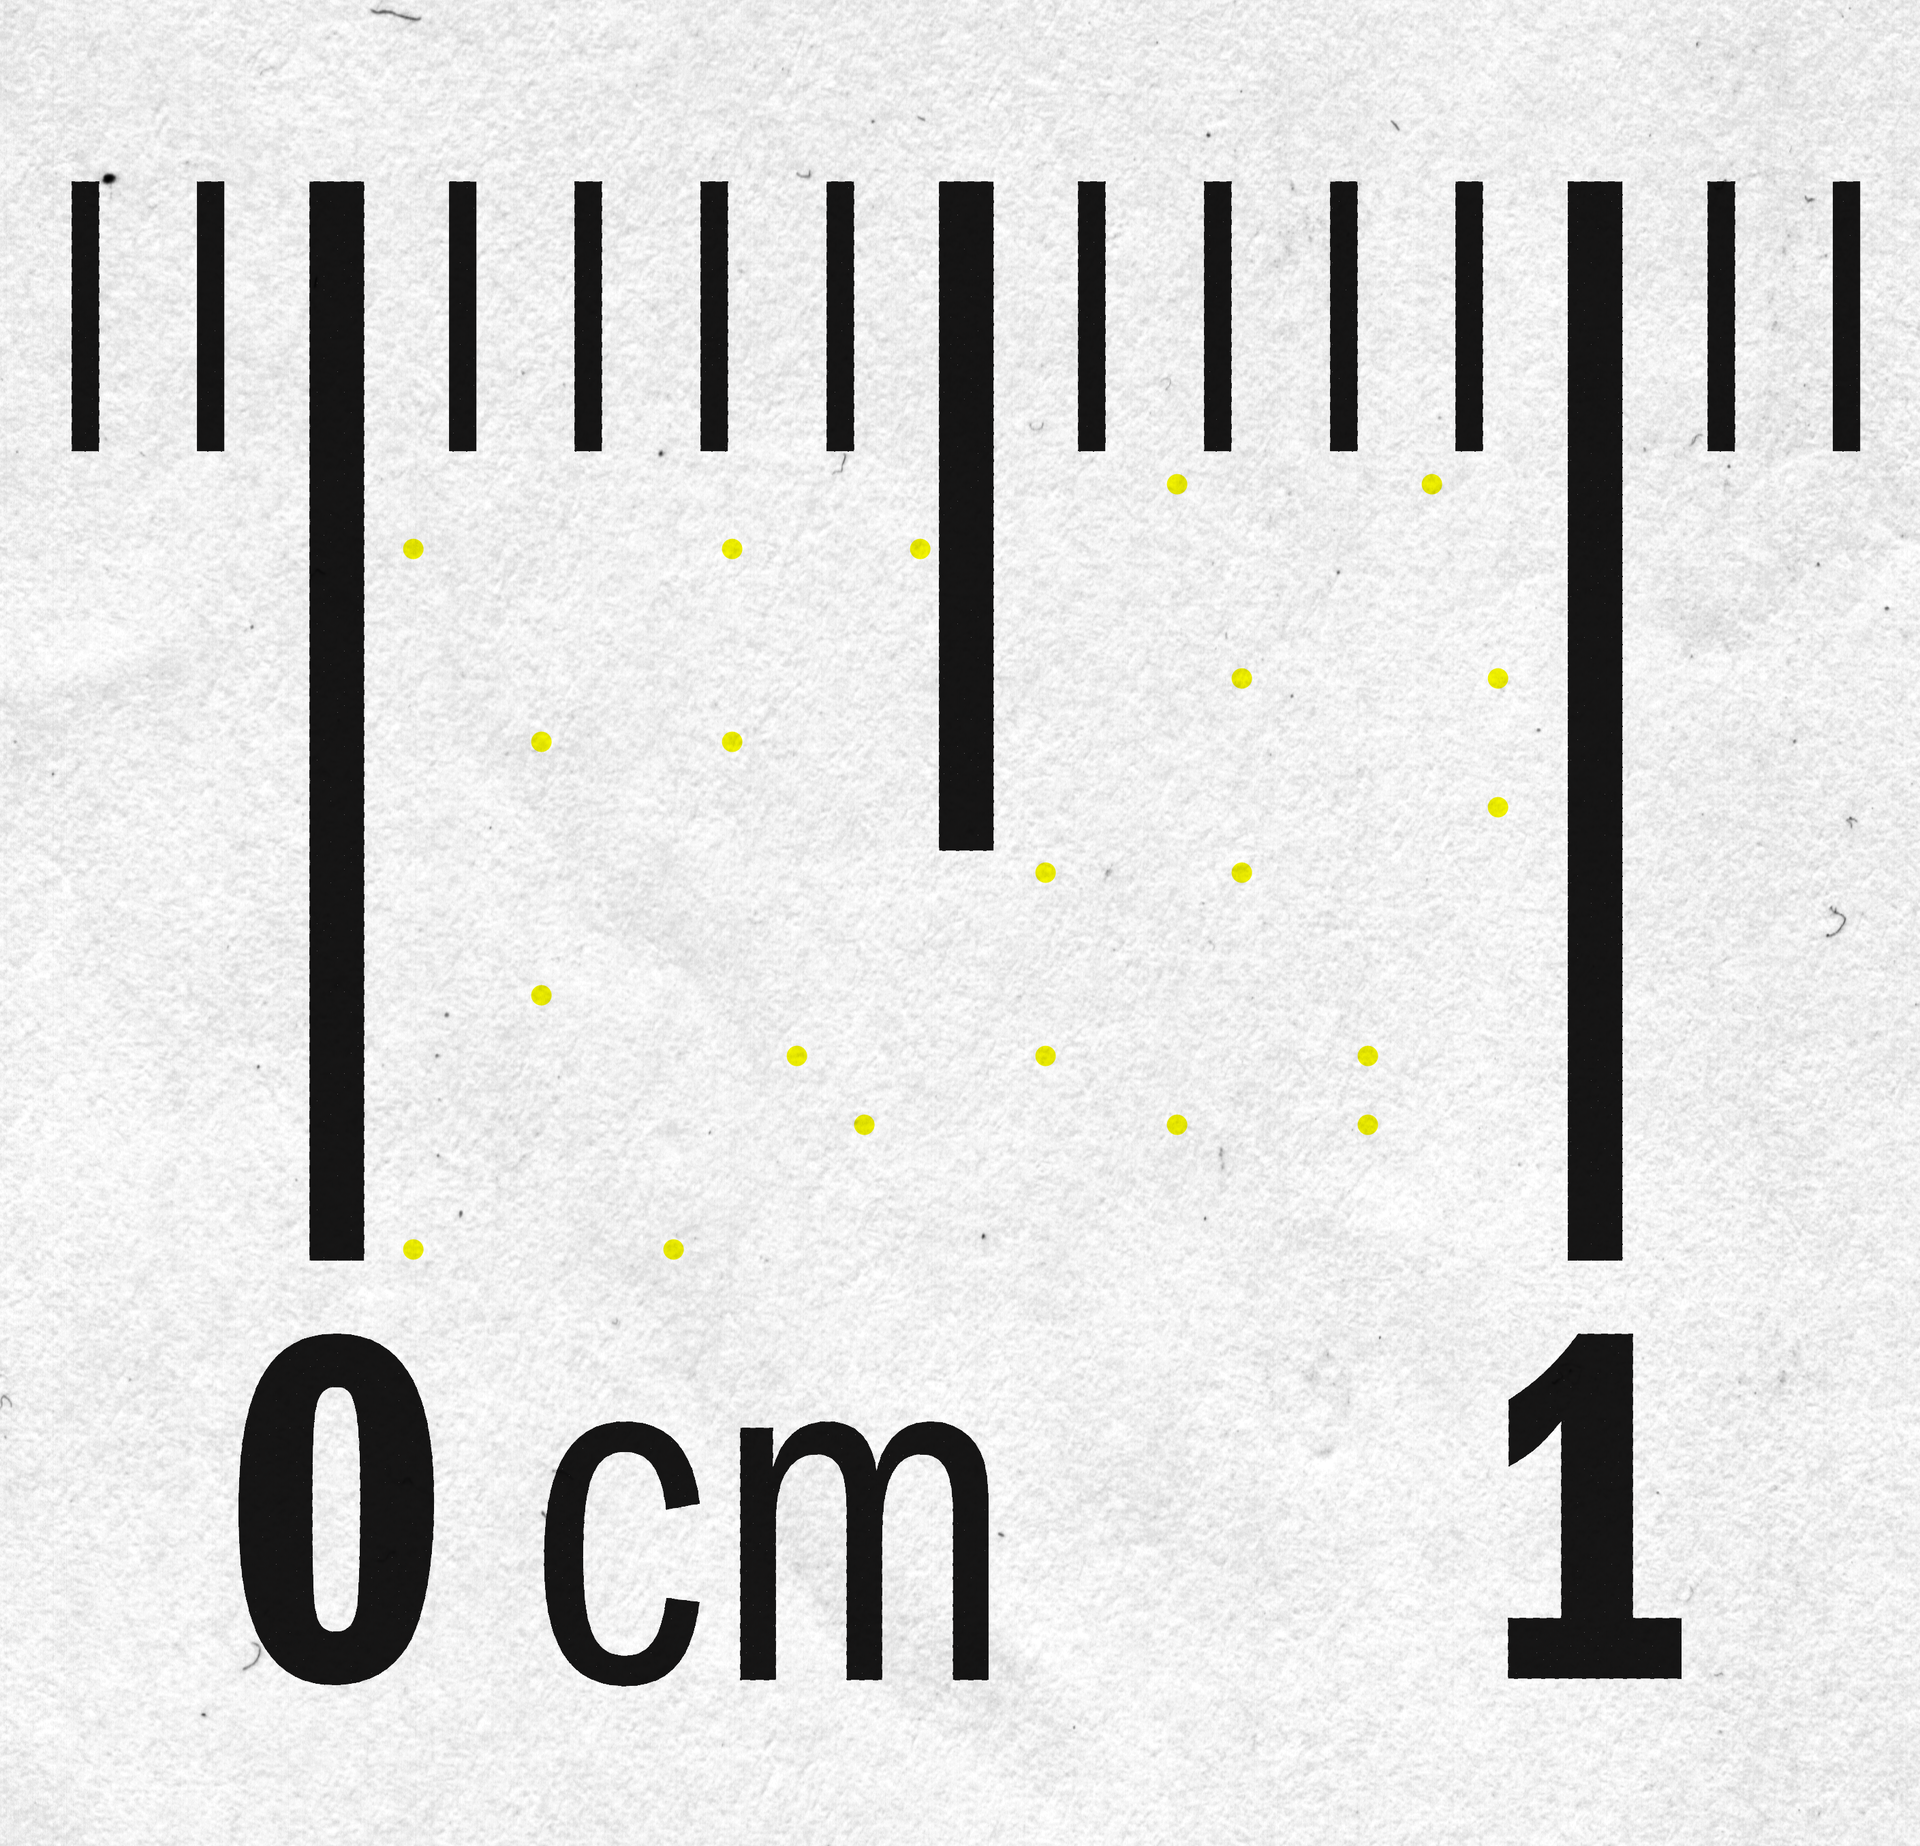
\includegraphics[width=5cm]{stego_drukarkowa}
	\caption{"kropki" zamieszczane przez drukarki}
\end{figure}
\begin{figure}
	\centering
	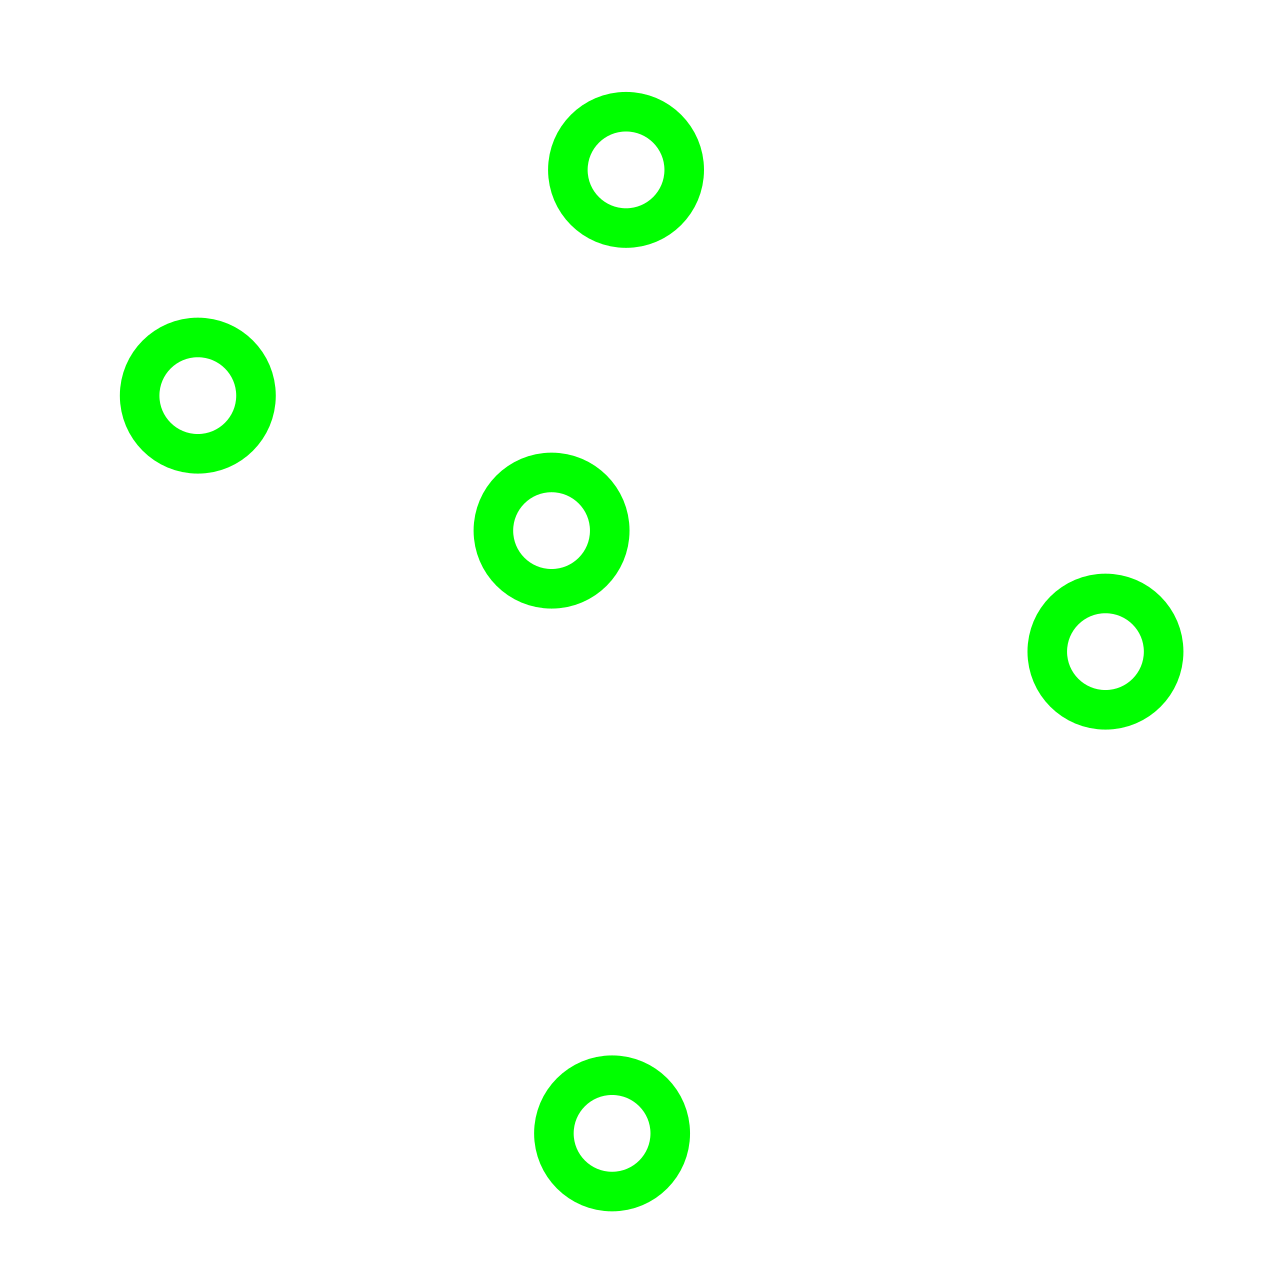
\includegraphics[width=5cm]{eurion}
	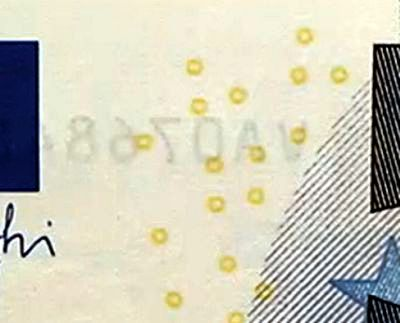
\includegraphics[width=5cm]{euro}
	\caption{EURion - układ kropek przypominających konstelację Oriona umieszczany na wielu banknotach}
\end{figure}
Steganografia może zatem realizować następujące funkcje bezpieczeństwa
\begin{itemize}
	\item poufność
	\item autentyczność
	\item niezaprzeczalność
	\item integralność
\end{itemize}
\section{Podział steganografii}
Ze względu na sposób ukrywania danych
\begin{itemize}
	\item steganografia czysta - nie jest stosowany żaden klucz, tekst jawny ukrywamy w pliku, jest to metoda 	Security through obscurity (nie spełnia zasady Kerckhoffsa)
	\item steganografia z kluczem prywatnym - przed komunikacją ustalany jest (np. algorytmem DH) klucz
	steganograficzny wykorzystywany potem w algorytmie, następnie ukrywamy tekst jawny w pliku
	\item steganografia z kluczem publicznym - w pliku ukrywamy szyfrogram zaszyfrowany kluczem publicznym
	odbiorcy
\end{itemize}
Ze względu na medium komunikacji
\begin{itemize}
	\item w plikach tekstowych
	\item w plikach audio
	\item w obrazach
\end{itemize}
\section{Słowniczek}

\section{Historia steganografii}
\section{Algorytmy steganografii w obrazach}
\subsection{Modyfikacja LSB}
\subsection{Gamma trick*}
\section{Algorytmy steganografii w plikach audio}
\section{Steganoanaliza}
\section{Źródła}
\begin{itemize}
	\item \url{https://pl.wikipedia.org/wiki/Steganografia_drukarkowa}
\end{itemize}

\end{document}
